\documentclass{standalone}

\usepackage{amsmath,amssymb}
\usepackage{tikz}

\DeclareMathOperator*{\argmin}{argmin}

\usetikzlibrary{shapes, arrows.meta, positioning, backgrounds}

\tikzstyle{block} = [rectangle, minimum width=1cm, minimum height=1cm, text centered, draw=black, fill=white]
\tikzstyle{circ} = [circle, minimum width=.5cm, minimum height=.5cm, text centered, draw=black, fill=white]
\tikzstyle{arrow} = [->,>=stealth]
\tikzstyle{line} = [-]

\begin{document}
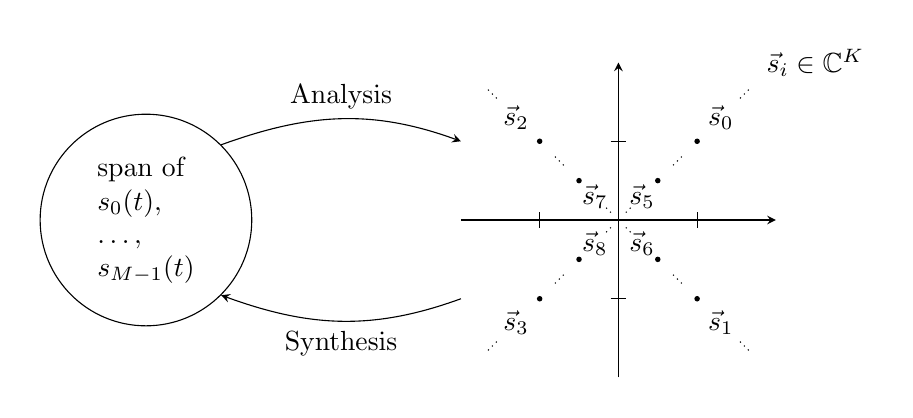
\begin{tikzpicture}[node distance=3cm, background rectangle/.style={fill=white}, show background rectangle]

    \node (span) [circ] at (-4, 0) {\begin{tabular}{l} span of \\ $s_0 (t),$ \\ $\ldots,$ \\ $s_{M-1} (t)$ \end{tabular}};

    \draw [arrow] (span.north east) to[out=20, in=160] node[anchor=south] {Analysis} (0, 1);
    \draw [arrow] (0, -1) to[in=-20, out=-160] node[anchor=north] {Synthesis} (span.south east);

    \node at (4.5, 2) {$\vec{s}_i \in \mathbb{C}^K$};

    \draw [arrow] (0, 0) -- (4, 0);
    \draw [arrow] (2, -2) -- (2, 2);

    \draw [line] (1, -0.1) -- (1, .1);
    \draw [line] (3, -0.1) -- (3, .1);
    \draw [line] (1.9, 1) -- (2.1, 1);
    \draw [line] (1.9, -1) -- (2.1, -1);

    \fill (3, 1) circle (1pt);
    \fill (3, -1) circle (1pt);
    \fill (1, 1) circle (1pt);
    \fill (1, -1) circle (1pt);

    \node at (3.3, 1.3) {$\vec{s}_0$};
    \node at (3.3, -1.3) {$\vec{s}_1$};
    \node at (0.7, 1.3) {$\vec{s}_2$};
    \node at (0.7, -1.3) {$\vec{s}_3$};

    \fill (2.5, 0.5) circle (1pt);
    \fill (2.5, -0.5) circle (1pt);
    \fill (1.5, 0.5) circle (1pt);
    \fill (1.5, -0.5) circle (1pt);

    \node at (2.3, .3) {$\vec{s}_5$};
    \node at (2.3, -.3) {$\vec{s}_6$};
    \node at (1.7, .3) {$\vec{s}_7$};
    \node at (1.7, -.3) {$\vec{s}_8$};

    \fill (2.15, .15) circle (.3pt);
    \fill (2.1, .1) circle (.3pt);
    \fill (2.15, -.15) circle (.3pt);
    \fill (2.1, -.1) circle (.3pt);
    \fill (1.85, .15) circle (.3pt);
    \fill (1.9, .1) circle (.3pt);
    \fill (1.85, -.15) circle (.3pt);
    \fill (1.9, -.1) circle (.3pt);

    \fill (2.8, .8) circle (.3pt);
    \fill (2.75, .75) circle (.3pt);
    \fill (2.7, .7) circle (.3pt);
    \fill (2.8, -.8) circle (.3pt);
    \fill (2.75, -.75) circle (.3pt);
    \fill (2.7, -.7) circle (.3pt);
    \fill (1.2, .8) circle (.3pt);
    \fill (1.25, .75) circle (.3pt);
    \fill (1.3, .7) circle (.3pt);
    \fill (1.2, -.8) circle (.3pt);
    \fill (1.25, -.75) circle (.3pt);
    \fill (1.3, -.7) circle (.3pt);

    \fill (3.65, 1.65) circle (.3pt);
    \fill (3.6, 1.6) circle (.3pt);
    \fill (3.55, 1.55) circle (.3pt);
    \fill (3.65, -1.65) circle (.3pt);
    \fill (3.6, -1.6) circle (.3pt);
    \fill (3.55, -1.55) circle (.3pt);
    \fill (.35, 1.65) circle (.3pt);
    \fill (.4, 1.6) circle (.3pt);
    \fill (.45, 1.55) circle (.3pt);
    \fill (.35, -1.65) circle (.3pt);
    \fill (.4, -1.6) circle (.3pt);
    \fill (.45, -1.55) circle (.3pt);

\end{tikzpicture}
\end{document}